
        \begin{abstract}{Thermo-physical Properties of Graphene Reinforced Thermoplastics: A Coarse- Grained Modelling Approach}{%
            R. Srivastava}{%
            Corso Duca degli Abruzzi 24, Turin, Italy}{%
            \IStag}
        Graphene, being one of the most promising material, has gained attention in scientific and industrial fields. With its superior properties, if introduced in the polymeric matrix can potentially improve material characteristics (such as thermal, elastic, electrical properties, etc). Thus, in this study coarse-grained molecular dynamic (CG MD) simulations were performed to investigate thermo-physical properties such as density, glass transition temperature, coefficient of thermal expansion, Young modulus, Poisson’s ratio and thermal conductivity of graphene reinforced thermoplastics (Polypropylene/graphene (PP/Gr) and Polylactic acid/graphene (PLA/Gr) composites).  Initially, we analyzed the thermo-physical properties of neat polymers (PP, PLA) and filler (Gr) using the MARTINI force field [1-2] and compared the results with experiments. Further, CG MD simulations were performed to determine the effect of graphene reinforcement on mechanical as well as thermal properties of PP/Gr and PLA/Gr composites. CG MD simulations show that Young modulus increases with increasing graphene concentration in the PP matrix, and in good agreement with experiments. Graphene reinforcement with $wt. = 2 \%$ increases the elastic modulus by $35 \%$ compared to neat PP. Similarly, enhancement of $12 \%$ in elastic modulus has been observed for PLA/Gr composite with similar reinforcements. We also performed the Non-Equilibrium Molecular Dynamic (NEMD) simulation to quantify the effect of graphene inclusion on the thermal properties of the composite using the Müller-Plathe algorithm [3]. In the case of the PP/Gr composite, effect of graphene concentration on thermal conductivity is negligible; whereas, a slight increase in thermal conductivity was observed in the case of PLA/Gr composite. The thermal behavior of composite is in agreement with literature values, which also show that the graphene concentration less than $5 \%$ wt. has negligible effects on the thermal properties of the composite [4].  \begin{center}  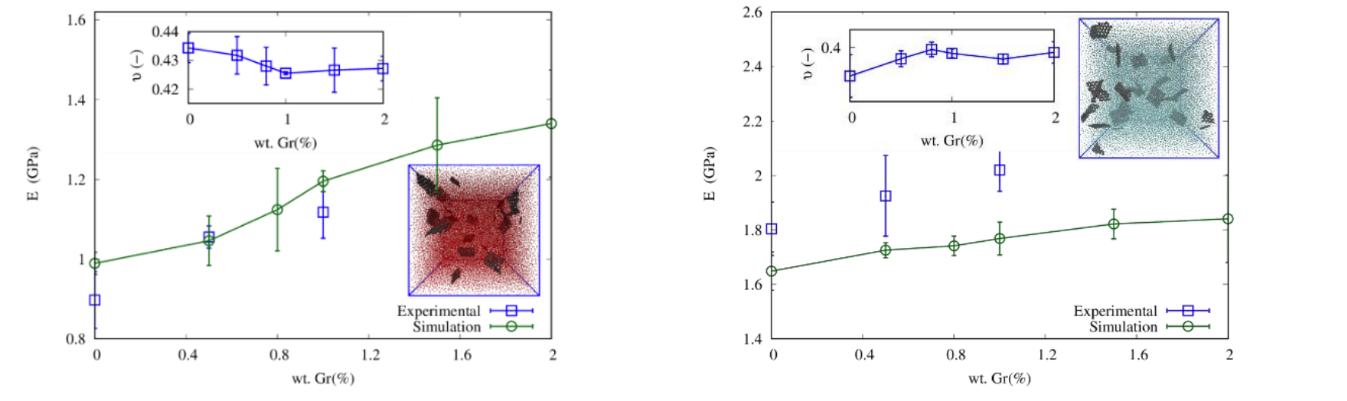
\includegraphics[width=\linewidth]{abstracts/txt/figures/rajat.png}  \caption{\textbf{Figure 1(a)} Young’s modulus (E) of PP/Gr composite as function of Gr $wt \%$. \textbf{(b)} Young’s modulus (E) of PLA/Gr composite as function of Gr $wt \%$.}  \end{center}  
        \end{abstract}
        